\documentclass[hidelinks,a4paper,12pt]{article}
\addtolength{\oddsidemargin}{-1.cm}
\addtolength{\textwidth}{2cm}
\addtolength{\topmargin}{-2cm}
\addtolength{\textheight}{3.5cm}
\newcommand{\HRule}{\rule{\linewidth}{0.5mm}}
\makeindex

\usepackage{longtable}
\usepackage[pdftex]{graphicx}
\usepackage{makeidx}
\usepackage{hyperref}
\hypersetup{
colorlinks=true,
linkcolor=black,
filecolor=blue, 
urlcolor=blue,
}


% define the title
\author{Not-Like-This}
\title{ Nimbus: AWS network visualiser}
\begin{document}
\setlength{\parskip}{6pt}

% generates the title
\begin{titlepage}

\begin{center}
% Upper part of the page 

\includegraphics[width=1\textwidth]{./images/up-logo.jpg}\\[0.4cm] 
\textsc{\LARGE Department of Computer Science}\\[1.5cm]
\textsc{\Large COS 301 - Software Engineering}\\[0.5cm]
% Title
\HRule \\[0.4cm]

\includegraphics[width=0.05\textwidth]{./images/logo.jpg} 
{ \huge \bfseries Amazon}

\includegraphics[width=0.05\textwidth]{./images/logo.jpg}\\[0.4cm] 
{ \huge \bfseries Network Visualizer}\\[0.4cm]
{ \huge \bfseries Demo 3}\\[0.4cm]
\HRule \\[0.4cm]
% Author and supervisor
\textsc{\Large Not-Like-This}\\[0.5cm]
\begin{minipage}{0.4\textwidth}
\begin{flushleft} \large
\emph{Authors:}
\end{flushleft}
\end{minipage}
\begin{minipage}{0.4\textwidth}
\begin{flushright} \large
\emph{Student number:}
\end{flushright}
\end{minipage}

\begin{minipage}{0.4\textwidth}
\begin{flushleft} \large
Jedd {Shneier}
\end{flushleft}
\end{minipage}
\begin{minipage}{0.4\textwidth}
\begin{flushright} \large
\emph{}
u13133064
\end{flushright}
\end{minipage}

\begin{minipage}{0.4\textwidth}
\begin{flushleft} \large
Daniel {King}
\end{flushleft}
\end{minipage}
\begin{minipage}{0.4\textwidth}
\begin{flushright} \large
\emph{}
u13307607
\end{flushright}
\end{minipage}

\begin{minipage}{0.4\textwidth}
\begin{flushleft} \large
Muller {Potgieter}
\end{flushleft}
\end{minipage}
\begin{minipage}{0.4\textwidth}
\begin{flushright} \large
\emph{}
u12003672
\end{flushright}
\end{minipage}

\vfill
% Bottom of the page
{\large \today}
\end{center}
\end{titlepage}
\footnotesize
%\input{declaration_of_originality.tex}
\normalsize


\pagenumbering{roman}
\tableofcontents
\newpage
\pagenumbering{arabic}


\section{Software Architecture Documentation}
\subsection{Vision} 
Amazon Web Services (AWS) is a comprehensive, evolving cloud computing platform provided by Amazon. 
AWS offers a suite of cloud computing services that make up an on demand computing platform. One such service is Amazon Virtual Private Cloud (Amazon VPC), which enables users to launch AWS resources into a virtual network. This virtual network closely resembles a traditional network. The problem is these networks are hosted logically on the cloud, and thus it is not immediately apparent how the network is structured. AWS customers have hundreds of inter-connected networks with tens-of- thousands of networked resources of many types and uses. Understanding the interplay of all these pieces, on a theoretical level, is no trivial task. In fact, is so difficult and tedious that most customers do not even bother fully understanding their services, leading to vastly complex and inefficient networks that pose serious security risks to companies.

The primary goal of this system is to provide an interesting and helpful tool to assist customers in understanding their own networks and how these networks can be improved and maintained. 
It is a network architecture tool, as well as a teaching tool, for the average user. The Network Visualizer is intended to be used by registered Amazon Web Services (AWS), in order to provide a simple and clear representation of the various networks' structures and thus, scan their entire network and depict the network in real time.

The system will take a valid pair of customer keys and connect to our application server, which will then make API calls to the aws ec2 API, to scan a users networks in different ways, with a variety of options. The scanned network will then be rendered back to the user as a interactive and dynamic network layout, that can be explored and played with to give them a clear understanding and an easy to understand visualization of complex logical connections and high level structures.

Finally, the system will be quite unique in scale and performance. Enormously large and complex networks will be scanned and visualized at extremely fast and efficient rates. The sheer scope of the data we work through and at the incredible performance gains we have developed over the traditional API calls is nothing short of astounding and we hope the thought and dedication to achieving this is accurately reflected in this document.

\newpage
\subsection{Architecture requirements}


\subsection{Architecture Scope}

\begin{enumerate} 
\item A secure key validation infrastructure: Highly sensitive data is sent by the user to the system, in the form of account keys which, if compromised, can result in massive financial damage. Thus, the handling of these sensitive data items is delegated to a specialised infrastructure to ensure their security.
\item A stable RESTfull infrastructure: Communication from the user interface to application is handled by a REST server architecture that handles requests, launches the requested scanners and updates the interface.
\item An easy to use user interface infrastructure: Users interaction with the system is important and thus there is an underlying architecture for handling their interaction and providing responsive output, in accordance with UI design paradigms.
\item A Scanner infrastructure to perform API calls: The main workhorse of the system comes down to scanning the users' networks. This is accomplished through the scanner architecture, which constructs specialised API calls to communicate with the AWS services and structures the responses from the calls. The entire architecture also follows a multi-threaded architecture design.
\item A centralized Buffer infrastructure: The "brain" of the system. The buffer serves as a connection for all the parts of the Application server. The threads are signalled through it, it constructs the scanned data into useful data artefacts that are visualized by the Visualizer and rendered to the user. The Buffer has several algorithms in place to construct the tree and connections.
\item A graphical Visualization infrastructure: The networks are rendered as hierarchical trees and dynamic node links. The the Visualizer infrastructure handles the update, drawing and interaction with the network tree and allows it to remain dynamic, attractive and smooth. It also handles the update of information, as the tree is iteratively produced in real time.
\item A tree persistence infrastructure: This part of the infrastructure handles the saving and retrieving of already scanned trees. This is useful in sharing of information and demonstrating to other parties the network structure.
\end{enumerate} 



\newpage
\subsection{Quality Requirements}
\subsubsection {Critical}
\begin{enumerate} 
\item Performance: The first and perhaps most important requirement. The system is working with massive amounts of data, as such the system is redundant if it can not process and show the data quickly. The majority of our architectural design has been implemented to improve performance, in order to keep it within its 3 second output requirement. Performance is measured in both time (how long it takes for functions to perform) and in terms of quality (do the functions perform adequate services to the user). We also tended to consider user performance, as in if the user struggles to get get useful information from the service in a reasonable time, then system has failed at that service. This is not a usability issue as the underlying goal of the system is to improve user performance in working with AWS networks.
\item Scalability: This is one of the major quality requirements for the service, as stated before. The system will have to work with very large networks in future and as such, the algorithms within will need to scale well; such that they can work with these large networks and so that performance costs are minimized. So far, our performance requirements matches our scale. Working with large data in an interconnected system like this, leads to several "bottlenecks". These bottlenecks are where parts of the system have not scaled as well as others and thus, cause delays in the execution of services. We have redesigned the architecture to address these bottlenecks and have put in place several safeguards to ensure that the slower parts do not impede the faster parts in any significant way. Where they do have an effect, the system able to handle other services in the waiting time. For this reason, we adopted a multi-threaded strategy when building our infrastructure.
\end{enumerate} 
\subsubsection {Important}
\begin{enumerate} 
\item Security: From our own experience, we know how important security is with this system. As we are working with sensitive client info (links to credit cards), it is imperative that we make sure the system is secure and does not allow for this information to fall in the hands of unwanted 3rd parties or be compromised in any way. This is less critical than the previous two requirements, as it is possible to secure on the client side however, we built this system without that assumption. 
\item Usability: Usability is very important, as ease of use is imperative to the client's experience. However, it is not as important as performance or scalability. At higher levels, regardless of usability, the system will be required to meet those requirements. The system is going to be used by the Amazon clients who will not necessarily have programming knowledge, thus the end product needs to cater to these users. The system is an effective teaching tool and if it is not usable or it cannot be understood easily, it is impossible to learn from using it.

\newpage

\item Reliability: With the hope that users will come to depend on the system, reliability is another chief concern. The system needs to remain stable and be consistent with its services. The built in safe guards to our architecture are intended to ensure that there is a very small probability of failures, and a minute frequency of errors.
\end{enumerate} 

\subsubsection {Nice To Have}
\begin{enumerate} 
\item Maintainability: The system will be handled over to Amazon and our hope is that with our documentation and architecture, it will be easily maintained. 
\item Extensibility: AWS is an ever changing and evolving platform and as new features are added, the system may need to be extended or changed. We have built the architecture with that in mind, to allow extensions.
\item Deployability: The system is intended to be deployed on an AWS instance and thus, the architecture has been designed to facilitate an easy deployment to this or any server.
\end{enumerate} 

\subsection{Access and integration channels}
\begin{enumerate} 
\item The system is hosted on AWS instance and accessed through standard HTTP access.
\item The Front end is integrated with the application API through a REST server using HTTP requests,AJAX and JSON responses.
\item The Application API is integrated with the Back-end Scanner via launching functions that associate with a Scanner thread. 
\item The Scanner threads are integrated with the Shared Buffer, via the SmartBuffer Interface and communicate through the buffer with thread signalling and NetworkTree objects.
\item The Scanner threads are also integrated with the AWS ec2 API. Calls to the API are made using tcp and responses are in JSON.
\item The interface is integrated with vis.js library, HTML 5, Bootstrap framework, Firefox, Google Chrome and Internet Edge
\end{enumerate}

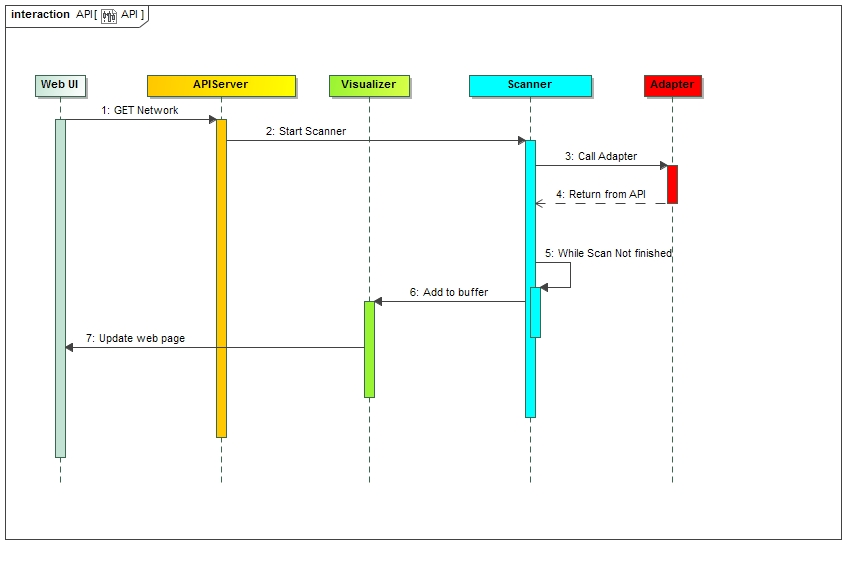
\includegraphics[width=1.00\textwidth]{./images/API.jpg}\\[0.4cm] 
\subsection{Architectural Constraint}
\begin{itemize} 
\item The System is mainly built in Java-EE with the user interface built in HTML5.
\item Styling of the user interface is accomplished through the Bootstrap Framework.
\item The REST server is built with the Jersey library.
\item Connection to the AWS ec2 API is done the AWS SDK for Java.
\item The Visualization engine is built using vis.js JavaScript library.
\item The system was built for and deployed on the Windows OS.
\item The system is deployed on an AWS T2 instance.

\end{itemize}
\newpage

\section{Architectural Design}
\subsection{Layered Architecture} 

Our core architectural design follows a standard Client-Application-Server layered architecture. As seen below, the "Server" (not to be confused with the Application server) is the AWS server we connect to through their API. The product does not persist to only read from it and we have no control over its functionality. It will be left for an integration requirement and will not be discussed further in this section. Additional information on the AWS system and their API can be found here: \url{https://aws.amazon.com/documentation/}. Previously, we used a bridging layer, (Adapter) to join the Application and Server layer, but it has since been incorporated into the Scanner, to reduce communication overhead and facilitate threading tactics. The primary back-end of the system lies on the Application layer, which is broken down into the several components.
\subsubsection{Application Layer}
Below are the central components of the Application Layer.
\subsubsection{Scanner}
The most important part of the system, the Scanner is the main focus for performance and scalability improvements. The central scan controller is managed through the Scanner Interface, which offers the following services:
\begin{enumerate} 
\item scanFullNetwork():Launches a scan of the entire network.
\item scanRegion(String region): Scans only the selected region.
\item scanNetworkFrom(String level, String identifier): Scans from the specified uuid.
\item scanUp(String level, String identifier): Scans up from the specified uuid.
\item scanAllInstnaces(): Scans all instanes in the network.

\end{enumerate}

To accomplish these services in a scalable and performance efficient way (depending on the services) a number of scanner threads will be launched. These threads are tasked with scanning a particular part of the network. See more below in Threading Tactic.
\newline
The concrete scanner ,AWSScanner, implements this interface. It has a built in Region scanner that scans all regions and launches an ec2 client for each region. These clients are assigned to each sub-scanner to make API calls and construct the node.
\newline
As the most important component, it constructs a scan based on different priorities. It forms a Producer-Consumer relationship with the Visualizer. Once launched, it will continue to produce network trees for the buffer until it receives a pause/stop command, or completes the specified scan.
\newline
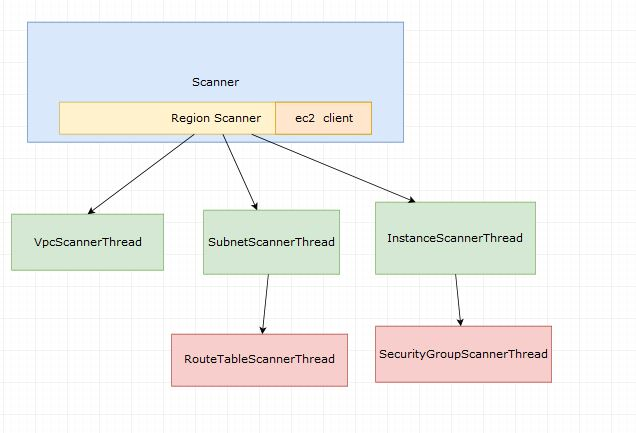
\includegraphics[width=1.00\textwidth]{./images/scanner.jpg}\\[0.4cm] 

\subsubsection{Buffer}
The link between the Visualizer and the Scanner Threads. The "brain" of the system. The individual scanner threads will add to the buffer as soon as they have finished constructing a tree, then go back to scanning. The trees arrive disjointed and possibly overlaps. The smart buffer constructs the entire network tree from the disjointed trees it receives. It stores the most up to date construct for the Visualizer. The buffer also stores node information that can be requested to send back the user.
\newline
Furthermore. the buffer also is the central message hub for all the threads. If the scanner state changes (stopped/paused/resumed), it is the buffer that signals all the threads. It is also responsible for knowing when all the threads are finished scanning. The buffer constructs relationships between instances, based on security group rules, and sub-networks based on route tabel rules. This is an extremely important requirement, as one of the problems facing many AWS users is the difficulty in determining what parts of the network can talk to what. This is important for both security and network architecture analysis.



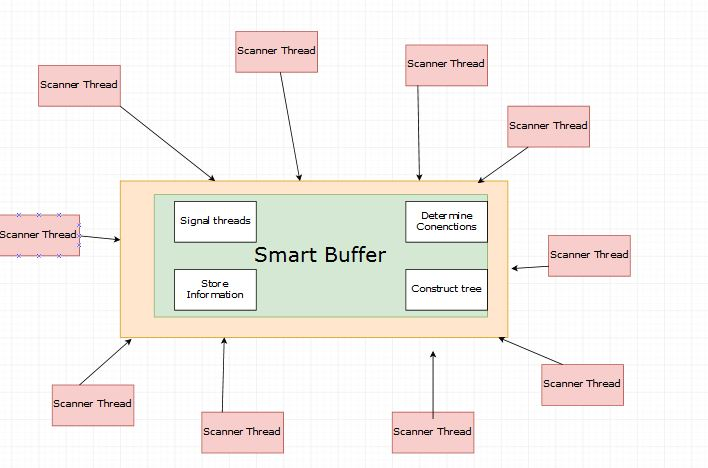
\includegraphics[width=1.00\textwidth]{./images/buffer.jpg}\\[0.4cm] 

\subsubsection{Client Layer}
The client layer consists of a Single Page Application and the Visualizer. The SPA is the user interface with all the scanning options, controls, the visualized graph and scanned information. The Visualizer polls on the REST server, requesting the latest tree from the smart buffer, rendering it and presenting it to the user. The Visualizer consists of a rendering engine to draw the graphic representation of the network, as well as a physics engine to allow interaction. 

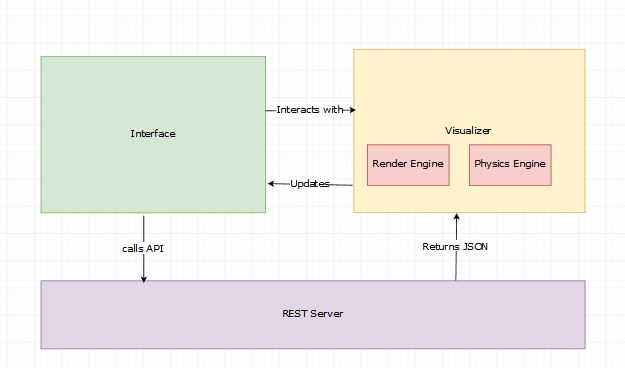
\includegraphics[width=1.00\textwidth]{./images/visualizer.jpg}\\[0.4cm] 


\subsubsection{Miscellaneous }
\begin{enumerate} 
\item Composite: Following the composite design pattern, this object represents the hierarchical Network tree, either in part or in whole. 
\item SecurityRuleSet: Contains security group rules for each instance determining what each instance  has permission to send too and receive from.
\item RouteTableRuleSet: Contains route table information for each sub-network, determining what each sub-network can talk too.
\item Parameter Beans: A number of communication and query beans used for sending information from client layer to server.
\item REST API and Server: The REST server joins the back-end to the front-end. See below.
\end{enumerate}

\includegraphics[width=1.00\textwidth]{./images/layered.png}\\[0.4cm] 
\newpage
\subsection{RESTFUL Design}

User interaction is mapped from the user interface onto different API calls on the server. Each call launches a back-end method to full fill the request. The API calls are:
\begin{enumerate} 
\item POST, validate: Takes the users' access and private key and creates a connection to AWS for the remainder of the session.
\item GET, startScanner: Launches a scan of the entire network, Visualizer polls on results as they stream in. 
\item GET, StopScan: Cancels the current scan.
\item GET, PauseScan: Pauses the current scan.
\item GET, ResumeScan:Resumes the current scan. Visualiser polls on buffer.
\item GET, ScanFrom: Performs a sub-scan starting from the given point and scanning around its general vicinity.
\item GET, ScanUP: Scans the next logical area above what the ScanFrom scanned.
\item GET, regionScan: Scans the specified Region only.
\item GET, scanAllIsntnaces: Scans every instance in the network only.
\item GET, getLatestTree: Requests the latest tree information from the buffer.
\item GET, getInformation: Requests the information for the specified node uuid.
\item GET, getConnection: Requests the connections for the specified node uuid.
\end{enumerate}

\subsection{Threading Tactic}
To improve performance and scalability, our system makes use of a number of threaded sub-scanners. Depending on service requested, the Scanner will launch a number of these scanners to fullfill the request in most efficient way possible.
\newline
This has led to exponential improvements. We keep the number of threads launched limited for hardware concerns. Each scanner thread has a single purpose and is focused on only one set of network components to scan. Each time a component is scanned, it is added to the shared buffer. The buffer handles thread signalling and synchronization. Each thread, when it is launched, takes a connection ticket from the buffer and when it is finished, it returns the ticket to the buffer to signal it has finished running. Depending on the network configuration, some threads may take for longer to finish than others, however the buffer keeps the visualizer notified so that the scan is not ended prematurely. By default, each region will launch one sub-scanner of each type, with certain sub-scanners launching sub-scanners of their own. 
The AwsScanner has a built in region scanner.
\newpage
The list of sub-scanners are below:
\begin{itemize} 
\item VpcScanner: Scans the Vpcs of a particular region.
\item SubnetworkScanner: Scans the sub-networks of a particular Region or Vpc.
\item InstanceScanner: Scans the instances of a particular Region, Vpc or Sub-network.
\item SecurityGroupScanner: Scans the security groups of each instance.
\item RouteTableScanner: Scans the route tables of each sub-network.
\end{itemize}



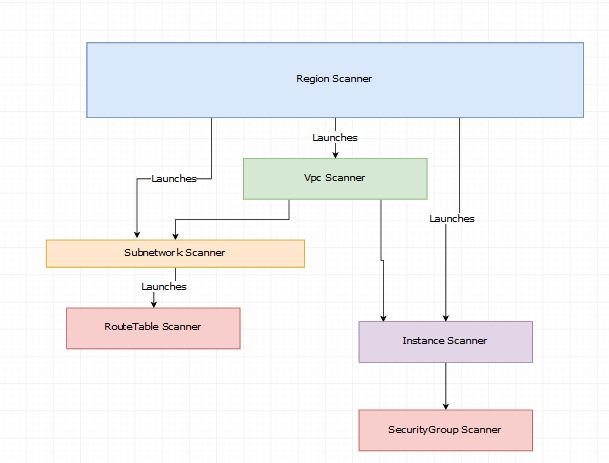
\includegraphics[width=1.00\textwidth]{./images/threads.jpg}\\[0.4cm] 

\newpage
\section{Reference architectures and frameworks }

\begin{itemize} 
\item Java Platform, Enterprise Edition: It offers a clean separation between behaviour and presentation for web applications. Thus, we can we can modularize our system into different layers and have each part handle its own services. This separation of duties allows for faster concurrent development as well as modular deployment and maintainability.
\item Bootstrap: This front-end framework offers us numerous resources to make a responsive interface. It was simple to integrate (as none of us are particularly skilled at web design). It was the simplest and cleanest way to improve our aesthetics.
\end{itemize}
\newpage
\section{Access and integration channels}

\subsection{Access channels}
Access to the system will happen through a web browser. The following web browsers are supported: Firefox, Google Chrome, Microsoft Edge. Users will HTTP to our server, hosted on an AWS T2 instance server. The server will retrieve our Single Page Applicationm called Nimbus. Through the Nimbus interface, a number of services can be called from our REST Server through HTTP and Ajax. Responses from the server will be in the form of JSON objects that will be visualized. 


\subsection{Integration Channels}
Our system will integrate externally with the aws ec2 API. It makes API calls through the Java AWS SDK using a tcp protocol. For more detailed information on the API calls used please see the official AWS API documentation at \url{http://docs.aws.amazon.com/AWSEC2/latest/APIReference/}
The following API calls are used:

\begin{enumerate} 
\item DescribeInstances: Describes one or more of your instances.
\item DescribeRegions: Describes one or more regions that are currently available to you.
\item DescribeRouteTables: Describes one or more of your route tables.
\item DescribeSecurityGroups: Describes one or more of your security groups.
\item DescribeSubnets: Describes one or more of your subnets.
\item DescribeVpcs: Describes one or more of your VPCs.
\end{enumerate}

\newpage
\section{Technologies} 
\begin{enumerate} 
\item Java SE 8u111
\item Java EE 7
\item Jersey 2.23.2 
\item aws-java-sdk-1.11.44
\item vis.js
\item HTML5
\item CSS3
\item Bootstrap
\item JavaScript
\item Windows 7 Ultimate Edition
\item HTML5
\item Google Chrome
\item Microsoft Edge
\end{enumerate}

\end{document}

